\documentclass[12pt,letterpaper]{article}

%Packages
\usepackage{amsmath}
\usepackage{amsthm}
\usepackage{amsfonts}
\usepackage{amssymb}
\usepackage{amscd}
\usepackage{dsfont}
\usepackage{enumerate}
\usepackage{fancyhdr}
\usepackage{mathrsfs}
\usepackage{bbm}
\usepackage{framed}
\usepackage{mdframed}
\usepackage{cancel}
\usepackage{float}
\usepackage{mathtools}
%\usepackage[]{mcode}
\usepackage{graphicx}
\usepackage{tikz}
\usetikzlibrary{automata,arrows}

%Page formatting
\usepackage[letterpaper,voffset=-.5in,bmargin=3cm,footskip=1cm]{geometry}
\setlength{\parindent}{0.0in}
\setlength{\parskip}{0.1in}
\allowdisplaybreaks
\headheight 15pt
\headsep 10pt

% Common Commands
\newcommand\N{\mathbb N}
\newcommand\Z{\mathbb Z}
\newcommand\R{\mathbb R}
\newcommand\Q{\mathbb Q}
\newcommand\lcm{\operatorname{lcm}}
\newcommand\setbuilder[2]{\ensuremath{\left\{#1\;\middle|\;#2\right\}}}
\newcommand\E{\operatorname{E}}
\newcommand\V{\operatorname{V}}
\newcommand\Pow{\ensuremath{\operatorname{\mathcal{P}}}}

\DeclarePairedDelimiter\ceil{\lceil}{\rceil}
\DeclarePairedDelimiter\floor{\lfloor}{\rfloor}

% 22 style
\newcommand\hint[1]{\textbf{Hint}: #1}
\newcommand\note[1]{\textbf{Note}: #1}
\newenvironment{22enumerate}{\begin{enumerate}[a.]\itemsep0em}{\end{enumerate}}
\newenvironment{22itemize}{\begin{itemize}\itemsep0em}{\end{itemize}}
\fancypagestyle{firstpagestyle} {
  \renewcommand{\headrulewidth}{0pt}%
  \lhead{\textbf{CSCI 0220}}%
  \chead{\textbf{Discrete Structures and Probability}}%
  \rhead{Klivans}%
}

\pagestyle{fancyplain}

\newcommand\EX{\mathds{E}}
\newcommand\PR{\mathds{P}}
\newcommand\zlam{Z_\lambda}
\DeclareMathOperator*{\argmin}{arg\,min}

\begin{document}
  \thispagestyle{firstpagestyle}
  \begin{center}
    {\large \textbf{Recitation 6}}
    
    {\large Computability}
  \end{center}
  
   \section*{Review}

	\textbf{Defn 1:} $\Pow{(S)}$ is the set of all subsets of $S$. 

	\textbf{Thm 1:} $|\Pow({S})| = 2^{|S|}$ if $S$ is of finite length. If $S$ is an infinite set then $|\Pow({S})| > |S|$.

	\subsection*{Warm-Up}
	
	Have you ever wondered what a computer is?

	One of the simplest models of computation is a \textbf{Deterministic Finite Automata} (DFA), which takes in an input string (usually a \textbf{binary string}) and either \textbf{accepts} or \textbf{rejects}.

	Here is how it works:
	\begin{itemize}
		\item Each ``circle" is a state with incoming and outgoing ``transitions". Start at the state that is labeled ``start".
		\item Read the input string from left to right. For each input character, follow the labeled transitions from the state you are currently in. This may take you to another state. 
		\item Once you have run out of symbols:
			\begin{itemize}
				\item If you are in a state with a double circle, \textbf{accept}. 
				\item If you are in a state with a single circle, \textbf{reject}.
			\end{itemize}
	\end{itemize}

	Consider the following DFA, which takes in a string of only 1's.

    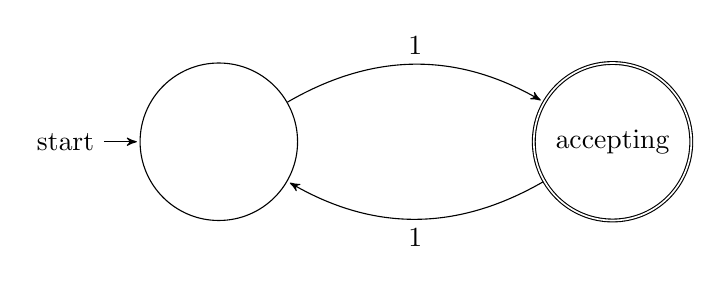
\begin{tikzpicture}[>=stealth',shorten >=1pt,auto,node distance=5 cm, scale = 1, transform shape]
    
    \node[initial,state,minimum size=2cm] (A)                                {};
    \node[state,accepting,minimum size=2cm]         (B) [right of=A]                       {accepting};
    
    \path[->] (A) edge [bend left]       node [above,align=center]  {$1$} (B)
			    (B) edge [bend left]       node [below,align=center]  {$1$} (A)
                
        ;
    
    \end{tikzpicture}

	For example, consider running the DFA on input ``1" . You first start in the left state, then see a ``1" and move to the right state. Therefore the DFA accepts ``1".
	\begin{enumerate}[a.]
	\item Does the DFA accept or reject the following strings:
	\begin{enumerate}[i.]
		\item ``11"
		\item ``111"
		\item ``11111"		
	\end{enumerate}
	\item What type of strings does this DFA accept? Prove your claim by induction on the length of the input string. 
	
	\begin{mdframed}
		\vspace{10cm}
	\end{mdframed}
	\item From now on we will only be considering DFA's which take \textbf{binary strings} as input. Consider the following DFA

    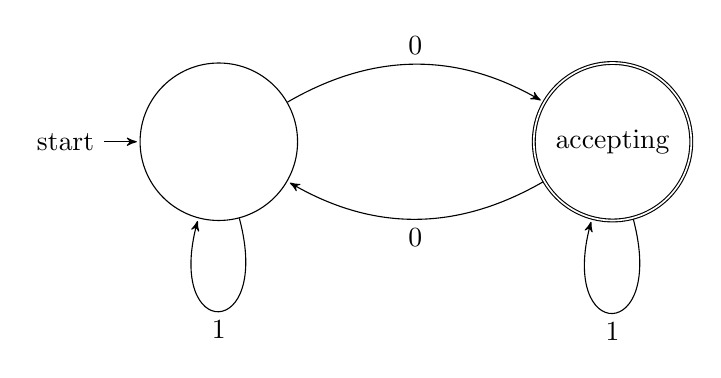
\begin{tikzpicture}[>=stealth',shorten >=1pt,auto,node distance=5 cm, scale = 1, transform shape]
	    \node[initial,state,minimum size=2cm] (A)                                {};
    \node[state,accepting,minimum size=2cm]         (B) [right of=A]                       {accepting};
    
    \path[->] (A) edge [bend left]       node [above,align=center]  {$0$} (B)
 				(A) edge [loop below]       node [align=center]  {$1$} (A)
			    (B) edge [bend left]       node [below,align=center]  {$0$} (A)
 				(B) edge [loop below]       node [align=center]  {$1$} (B);
	\end{tikzpicture}	
	
	Let $L$ be the set of strings accepted by this DFA. Which of the following is correct:
	\begin{enumerate}[i.]
		\item $L = \{ w \ | \ w \text{ is a binary string of even length}\}$
		\item $L = \{ w \ | \ w \text{ is a binary string with an odd number of 0's}\}$
		\item $L = \{ w \ | \ w \text{ is a binary string with an odd number of 1's}\}$
	\end{enumerate}

	\item Let $\Sigma$ denote the set of 0/1 strings of any length. Is this set infinite?

	\item Consider an arbitrary input $w$ to a DFA. Circle all of the correct statements below.
	\begin{enumerate}[i.]
		\item $ w \subseteq \Sigma $
		\item $ w \in \Sigma $
		\item $ \{w\} \in \Pow({\Sigma}) $
	\end{enumerate}

	\item The \textbf{language} $L$ of a DFA is the set of strings which the DFA accepts. Circle all of the correct statements below.
	\begin{enumerate}[i.]
		\item $ L \subseteq \Sigma $
		\item $ L \in \Sigma $
		\item $ L \in \Pow({\Sigma}) $
	\end{enumerate}
	
	\item Design a DFA that accepts a binary string if it ends in a 0. For example, the string ``100" is accepted and the string ``1101" is rejected.

	\begin{mdframed}
	\vspace{7cm}
	\end{mdframed}

	\item Design a DFA that only takes in strings consisting of 1's and accepts a string only if it is a multiple of 3. (Note that 0 is a multiple of 3)

	\begin{mdframed}
	\vspace{7cm}
	\end{mdframed}

	\end{enumerate}

	\section*{Section Lesson - The Limit of Computation}

	\subsection*{Is there anything a computer can't do? (Set Proof)}

	Our complete model of computation is called a $\textbf{Turing Machine}$ after Alan Turing. We call it complete because a Turing Machine can do everything a computer program can do. It is very similar to a DFA and either accepts or rejects a binary string. 

	A turing machine has a language $L$ of binary strings it accepts.

	\begin{enumerate}[a.]
		\item How many languages are there? Write your answer in terms of $|\Sigma|$, $|\Pow(\Sigma)|$ and explain.
		\begin{mdframed}
		\vspace{4cm}
		\end{mdframed}
		\item Like a computer program, a Turing Machine can be represented as a 0/1 string. How many Turing Machines are there? Write your answer in terms of $|\Sigma|$, $|\Pow(\Sigma)|$ and explain.
		\begin{mdframed}
		\vspace{1.6cm}
		\end{mdframed}
		\item What can you conclude from this? Can you build a computer program / Turing Machine for every language?
		\begin{mdframed}
		\vspace{1.6cm}
		\end{mdframed}
 	\end{enumerate}

	\subsection*{Side Note - History}
From Wikipedia: ``Turing is widely considered to be the father of theoretical computer science and artificial intelligence." During the second world war, ``Turing played a pivotal role in cracking intercepted coded messages that enabled the Allies to defeat the Nazis in many crucial engagements". Despite this, he was prosecuted as a criminal for homosexual acts and commited suicide in 1952 at age 41.

	\subsection*{Proof by Contradiction - \textit{Optional Challenge Problem}}

	\textit{This is confusing and is far beyond the scope of CS22, only read on if you are interested. This is not meant to be part of recitation.}

	Let $P$ be a computer program. $P(\omega)$ means that we are running the program $P$ on input $\omega$. Both a program and its input can be represented as a 0/1 string. This means that we can run a program on itself, written as $P(P)$. 

	$P(\omega)$ can either terminate or enter an infinite loop. It would be helpful if we had another program, $HALT$, which would take as input $P(\omega)$ that would tell us if $P(\omega)$ would terminate or not.

	You will show that $HALT$ cannot exist with a proof by contradiction.

	Assume for sake of contradiction that $HALT$ exists.

	Using $HALT$ which we have assumed exists, we can build the program $OPPOSITE$. $OPPOSITE$ does not output anything, it either terminates or loops forever. $OPPOSITE$ takes as input a program $P$ and executes the following steps:
	\begin{enumerate}[(1)]
		\item Run $HALT$ on $P(P)$.
		\item If $HALT$ says that $P(P)$ loops forever, then terminate.
		\item If $HALT$ says that $P(P)$ terminates, then loop forever.
	\end{enumerate}

	Since $OPPOSITE$ takes a computer program as input, we can run it on itself.

	Consider running $OPPOSITE$ on $OPPOSITE$.

	\begin{enumerate}[a.]
		\setcounter{enumi}{3}
		\item Can $OPPOSITE(OPPOSITE)$ halt?
		
	\hint{If $OPPOSITE(OPPOSITE)$ halts, then what happens in step 2 of $OPPOSITE$? Is this a contradicition?}

			\begin{mdframed}
		\vspace{3.6cm}
		\end{mdframed}

		\item Can $OPPOSITE(OPPOSITE)$ loop forever?

	\hint{If $OPPOSITE(OPPOSITE)$ loops forever, then what happens in step 3 of $OPPOSITE$? Is this a contradicition?}

		\begin{mdframed}
		\vspace{3cm}
		\end{mdframed}

	\item Have we reached a contradiction? Why? If so we know that the $HALT$ program cannot exist.

		\begin{mdframed}
		\vspace{3cm}
		\end{mdframed}
	
	\end{enumerate}
	

	



	

	

	

	
	
  

\end{document}